\section{ESMF Classes}

We divide the ESMF classes into three main categories: those associated 
with the coupling superstructure, those associated with the data handling
infrastrucure, and those that are part of the utility layer.  
Superstructure and Infrastructure
classes are based on a hierarchical 
calling tree of increasingly abstract data structures that represent the field data associated 
with the physical systems being modeled.  
Superstructure classes provide methods which invoke user-supplied code;
Infrastructure classes provide methods which are invoked by
user-supplied code.
Utility classes are independent 
of the data classes, though they too have a hierarchical structure; 
higher-level utilities employ general-purpose tools such as a message log.

In the listing of classes below we provide a description of each class and its function.

\subsection{Object Model}

The hierarchy of classes in ESMF is shown in the following UML diagrams.  

\subsection{Components}

The top level object in the system is a Component object.
Types of components are shown in the diagram below:

\scalebox{0.70}{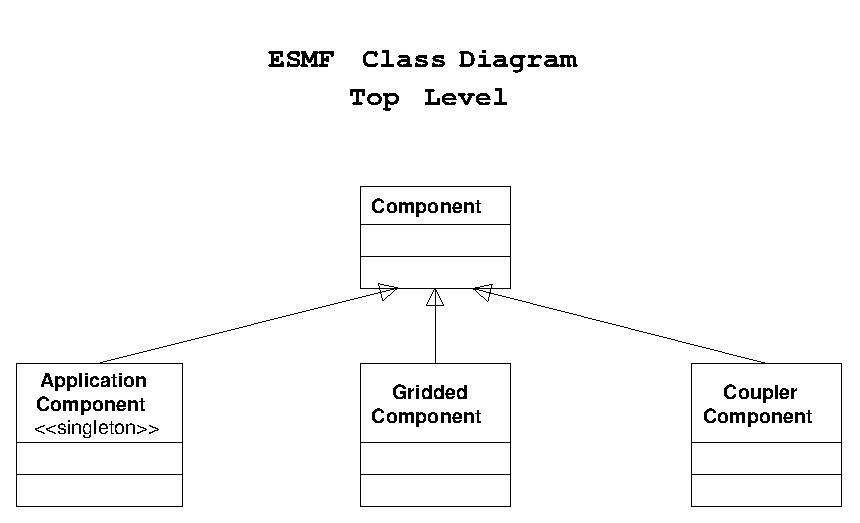
\includegraphics{ESMFTopClassDiagram.eps}}

Detailed descriptions of these objects are:

\subsubsection{Component (ESMF\_Comp)} 
\begin{description}
\item [Description] A Component is a functionally related computational entity that represents 
a large system.  
% \item [Function]  ...
\end{description}

\subsubsection{Application (ESMF\_App)}
\begin{description} 
\item [Description] We define an Application (ESMF\_App) as a special kind of Component 
that is itself composed of a set of sub-Components that interact to form a complete scientific
application.  
\item [Function] The ESMF\_App class is responsible for managing those functions that relate 
to an entire scientific application running under ESMF.  The ESMF\_App initialize method 
must be called at the start of any user application operating under the framework, and
the ESMF\_App finalize method at its end.  At initialization the Application allocates and 
configures any resources needed to run the framework.  The Application also specifies whether 
the system will be brokered using the Registry or not.  The ESMF\_App class can be queried 
for information such as an experiment name, model name, run type (ESMF\_INIT, 
ESMF\_BRANCH, etc.), and for an overall Status.  It can also be queried for
information on any Component that it includes, including its Name, Map, and
Status.
\end{description}

\subsubsection{Coupler Component (ESMF\_Coupler)}
\begin{description}
\item [Description] A Coupler is a specialized type of Component that encompasses all the 
functionality needed to communicate data between two or more Components. 
\item [Function] A Coupler must have methods to register new Components, to negotiate
which Components need to exchange data, with optional Transformations of data, and to
mediate the actual data exchange.
\end{description}

\subsubsection{Transform (ESMF\_XForm)} 
\begin{description}
\item [Description] A Transform takes one or more physical quantities defined using one set 
of units or representation and translates them as needed to a different set of units or 
representation, for example, potential temperature to temperature.  Transform objects 
are specialized by the application developer.
\item [Function] The Transform class is an abstraction introduced for the
purpose of standardizing high-level coupling interfaces.  It may be overloaded
to take sets of individual Fields or Bundles.  Methods may include a
separate initialization and run. 
\item [Note] << this object was in the text here, but doesn't
exist in the corresponding diagram.  which one needs to be fixed?? >>
\end{description}

\subsubsection{Gridded Component (ESMF\_GComp)}
\label{sec:griddedcomponent} 
\begin{description}
\item [Description] A Gridded Component is a specialized type of Component that is associated
with computational data and the grid on which it is located.
\item [Function] The GComp class is an abstraction to unify the grid and data carrying
objects in the system: the Grid class, the Field class, and the Bundle class.
<< what common Methods are at this level?? >>
\end{description}


\subsection{Application}

<< needs text here >>

\subsection{Coupler}

This diagram shows the flow of control between two Gridded Components
mediated by and interacting with the Coupler component: 

\scalebox{0.70}{\includegraphics{ESMF_coupler.eps}}

\subsection{Transform}

<< needs text here >>

\subsection{Gridded Components}

Gridded Components encapsulate the computational data and the
grid on which it is located.  A Gridded Component contains
the following object hierarchy:

\scalebox{0.70}{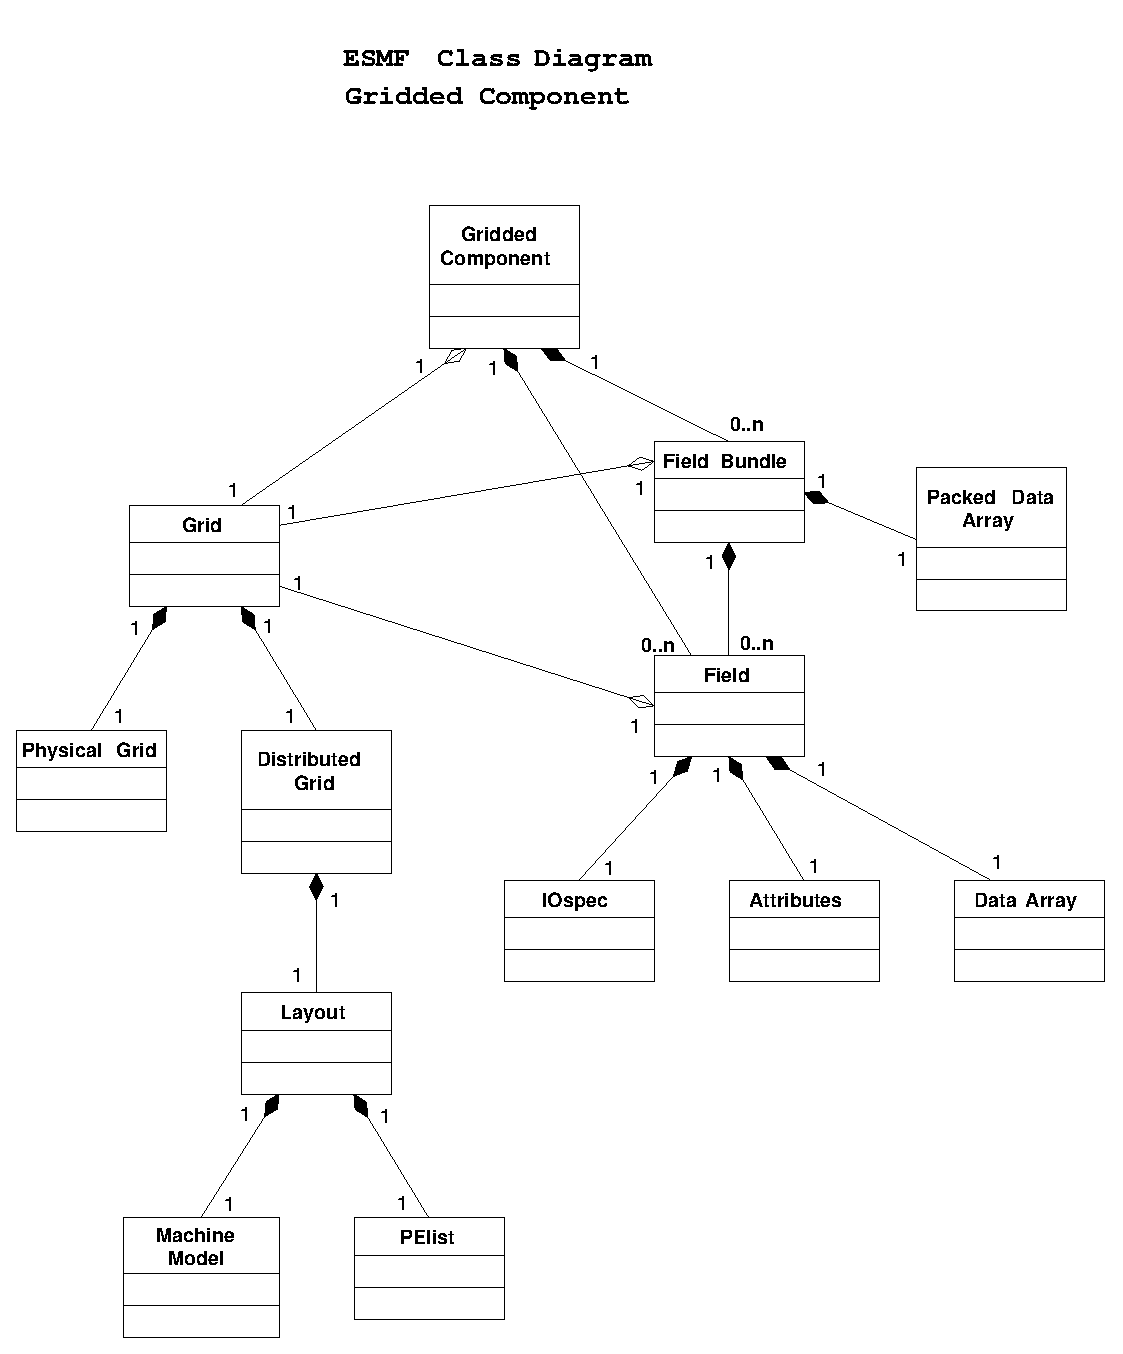
\includegraphics{ESMF_DataStructureHierarchy.eps}}


\subsubsection{Bundle (ESMF\_Bundle)}
\label{sec:bundle} 
\begin{description}
\item [Description] A Bundle contains one or more Fields which are defined on the
same Grid.  It allows the application to manipulate multiple fields in an identical
manner with a single set of calls.  It also allows the option of interleaving data
from multiple fields into a Packed Data Array (see Section~\ref{packeddataarray}) for
more efficient memory access patterns.
\item [Function] The Bundle class is an aggregation of the Field class.  It provides methods 
for getting and setting fields.  It provides methods for querying information about the
underlying grid.  It provides methods for requesting the packing of data, the
reordering of that packed data, and detaching and attaching the data.
\end{description}

\subsubsection{Packed Data Array (ESMF\_PackedData)}
\label{sec:packeddataarray} 
\begin{description}
\item [Description] A Packed Data Array contains data from one or more Fields, where the
data items are interleaved in memory. The application may use a packed array to maintain
locality of reference while iterating the array, or for ease in subsetting multiple
data values in one operation.
\item [Function] The PackedData class provides methods for packing and querying arrays,
subsetting the data, and repacking the data in a different order.  The PackedData object
contains an Ordering object to maintain the information about the structure of the packing.
It is contained by a Bundle object.  Application access is through Bundle methods.
\end{description}

\subsubsection{Field (ESMF\_Field)}
\label{sec:field} 
\begin{description} 
\item [Description] A Field represents a single physical field or the components of a 
vector field.  It is the basic data carrying object in the system.  It includes both
the data and the grid on which the data is defined.  The main application interfaces
for accessing data are here.
\item [Function] The Field object is a composition of the Data Array object, an optional
Mask object, an optional IOspec object, and it aggregates a Grid object.  It provides
methods for getting, setting, and querying the data array, the grid, the mask and
the I/O spec.  It provides methods for detaching and attaching data from the field.
While data is detached it is the responsibility of the application.  A Field object
provides methods for subsetting, regridding, and reordering memory layout of data.
\end{description}

\subsubsection{Mask (ESMF\_Mask)}
\label{sec:mask} 
\begin{description}
\item [Description] A Mask describes a subset of data items, for example to indicate
the valid values which represent ocean points (and not land) in an ocean model.  
It may be specified at the Grid object level, but it is stored below the Field level 
for effiency of computation.
\item [Function] The Mask class is an optional part of a Field class.  It provides methods
for getting and setting valid values.
\end{description}

\subsubsection{Data Array (ESMF\_Data)}
\label{sec:dataarray} 
\begin{description}
\item [Description] A Data Array is a list of data values plus information about
the data itself.
\item [Function] The Data class contains the data as well as information about the data,
including the data type (e.g. float,
integer), the machine type (e.g. IEEE float, Cray float), data count, data dimensionality
(e.g. scalar, vector).  It provides methods for querying all information about the data,
returning a pointer to the memory location of the start of the data, and conversion routines
for altering the characteristics of the data.  Information about how the data array is laid
out in memory is contained in an Ordering class.
\end{description}

\subsubsection{Ordering (ESMF\_Ordering)}
\label{sec:ordering} 
\begin{description}
\item [Description] A Ordering is the description of how multidimentional data have been
linearized in memory.  This includes both multidimensional array index information (e.g. C-order
vs Fortran-order) as well as vector or tensor data item information (e.g. all Xs then all
Ys vs [X,Y], [X,Y] tuples).
\item [Function] An Ordering object is associated with a single Data object.  It provides
methods to query the current memory organization and methods to reorder the Data object.
\end{description}

\subsubsection{Grid (ESMF\_Grid)}
\label{sec:ordering} 
\begin{description}
\item [Description] A Grid is the general representation of the coordinate information for
the computation.  It contains both the logical presenatation of the grid as well as the
decomposition of the grid into subgrids for processing in parallel on a
multiprocessor system.
\item [Function] The Grid class is the composition of a PhysGrid and a DistGrid object.  
It is aggregated into the Field and the Bundle objects.  It provides methods to the
Field and Bundle classes for obtaining coordinate, indexing, and decomposition information.
\end{description}

\subsubsection{Physical Grid (ESMF\_PhysGrid)}
\label{sec:physgrid} 
\begin{description}
\item [Description] A Physical Grid is a discrete representation of a continuous physical space.
There are a multitude of types of physical grids.
The grid contains the physical coordinates, usually indicating where data values are located, but
it could be a parametric description of the actual locations.  
\item [Function] The PhysGrid class maintains a global index space for coordinate information.
It provides methods for creating a variety of grid types, including both reading grid information
and generating grids from parameters.  It provides methods for regridding, or translating
one grid to another, used for example when exchanging data through the coupler between
various components.
The PhysGrid class does not handle grid decomposition issues related to 
distributed processing; see the Distributed Grid object in Section~\ref{distgrid}.
\end{description}

\subsubsection{Distributed Grid (ESMF\_DistGrid)} 
\label{sec:distgrid} 
\begin{description}
\item [Description] A Distributed Grid is a collection of subgrids which
constitute a single logical grid.  The subgrids can be operated on in
parallel on a multiple processor machine.  
\item [Function] The DistGrid class contains the mapping
between the local grid decompositions and the global logical grid. 
It contains methods to 
synchronize data values between the boundaries of subsets, and to
collect and communicate global data values.  It interacts closely with
the Physical Grid object (see Section~\ref{physgrid}).
It uses a Layout object to identify and manage the processing elements 
available for the computation.
\end{description}

\subsubsection{Original Layout (ESMF\_Layout)}
\label{sec:olayout} 
\begin{description}
\item [Note] << This is the original description in the doc; i've updated
it below.  comments?? nsc. >>
\item [Description] A layout is a description of a computational domain that
may describe the decomposition of an Application, a Component, a Field Group, a Field, or 
a Distributed Grid.
If no Layout is specified for an object, it can inherit its layout from an object
higher in the data hierarchy.  
\item [Function] The Layout class ...
\end{description}

\subsubsection{Layout (ESMF\_Layout)}
\label{sec:layout} 
\begin{description}
\item [Description] A Layout is a description of the decomposition of
a Distributed Grid across multiple physical processors or processing elements.
A single Distributed Grid can have multiple Layouts, each describing a different
logical decomposition for different purposes.
\item [Function] The Layout class maintains the mapping of 
subsets of the entire logical grid to processing elements.
\end{description}

\subsubsection{Processor Element list (ESMF\_PElist)}
\label{sec:pelist} 
\begin{description}
\item [Description] A Processor Element list contains a list of Processing Elements (PEs) 
available to participate in the computation.  It includes a unique identifier for each PE, 
information about what memory or communication groupings it belongs to (e.g. subsets 
of PEs which share the same physical memory), and other identifiers for virtual resources.  
\item [Function] The PElist class encapsulates information needed to schedule
jobs in parallel, and is aggregated into the Layout class (see Section~\ref{layout}).
It provides query methods to the Layout object, and some limited query methods
may be available at the application level.
\end{description}

\subsubsection{Machine Model (ESMF\_MachineModel)}
\label{sec:machinemodel} 
\begin{description}
\item [Description] A Machine Model describes the characteristics of memory and
communication characteristics which influence choices for accomplishing a parallel 
decomposition of a large problem.  For the most part the application does not
interact with this class of object, although some query routines are provided.
\item [Function] The MachineModel class encapsulates all hardware dependent information
about the memory subsystem (e.g. physical shared memory, distributed shared memory, clustered
memory), what communication transport mechanisms are available (MPI, OpenMP, etc), 
whether the processors are homogeneous or heterogeneous, and 
any other relevant hardware information (e.g. processor speed).
It is aggregated into the Layout class (see Section~\ref{layout}), and provides
methods for querying all characteristics needed by the Layout object to do 
problem decomposition and distribution of work.
The MachineModel class does expose some limited query methods to the application, 
to allow for the possibility of making run-time choices of algorithms based on hardware type.
\end{description}

\subsubsection{Input/Output Specfication (ESMF\_IOspec)}
\label{sec:iospec} 
\begin{description}
\item [Description] A Input/Output specfication contains all information necessary to
read or write objects.  It includes the destination information (e.g. file), the name,
the format, and any format specific parameters needed to complete the I/O.
\item [Function] The IOspec class is ...   << how does this fit?? >>
\end{description}


\subsection{ESMF Base Object}

All objects above are based on the object below.  Attributes
can be handled by generic routines, but it is expected that 
higher level objects will supply their own class specific
methods of the ones listed below.

\scalebox{0.70}{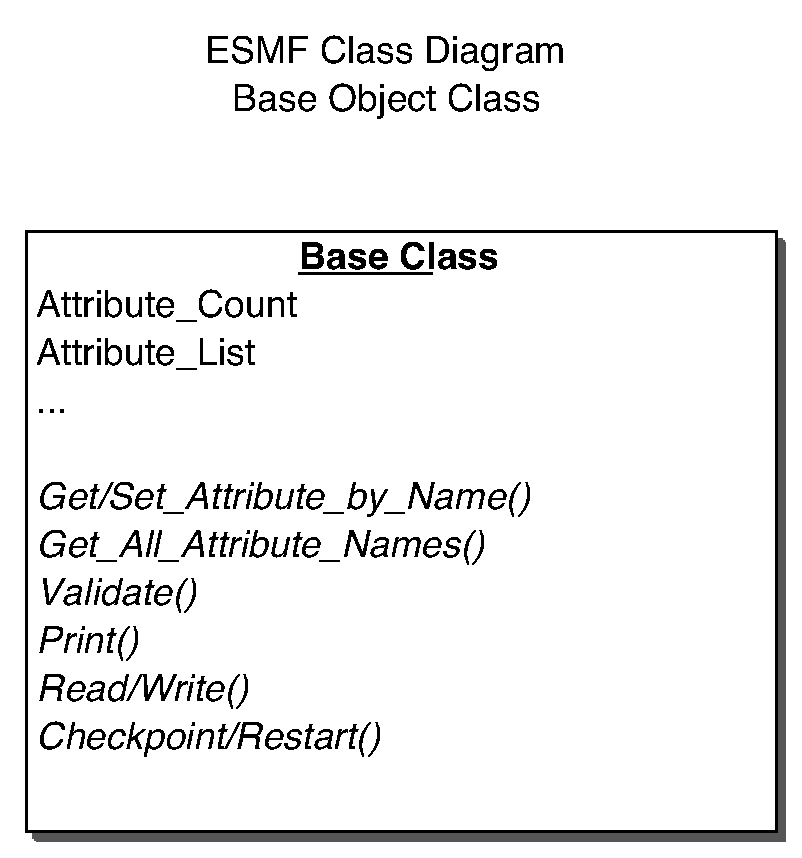
\includegraphics{ESMF_Base.eps}}

\subsubsection{Base (ESMF\_Base)}
\label{sec:Base} 
\begin{description}
\item [Description] The ESMF Base class is an abstraction of the private data and
methods common to all other object in the system.  Some methods and data can be
inherited direcly from the Base class; others are expected to be overloaded by
higher level objects.
\item [Function] The Base class methods which are expected to be overloaded by
more specialized objects include: Print, Validate, Read/Write, Checkpoint/Restart.
Methods which are inherited by all other classes include those which 
set and query object Attributes.
\end{description}

<< perhaps the usage section goes here, or perhaps this doesn't
belong here and does belong combined with the usage section >>

\subsection{Utility Level Objects}

\subsubsection{Basic Utilities (ESMF\_BasicUtil)} 
\begin{description}
\item [Description] Utilities that may be utilitized by any other class in the ESMF.  
Collecting these functions into a base-level utility set helps to 
avoid circular referencing.
\item [Function] 
\end{description}

\subsubsection{Basic Communications (ESMF\_BasicComm)}
\begin{description}
\item [Description] This library is a wrapper for MPI and other vendor-supplied 
message passing libraries.
\item [Function] The Basic Communication library provides a generic interface
and efficient communications for the ESMF.  Methods include scatter, gather, send,
receive, synchronize. 
\end{description}

\subsubsection{ (ESMF\_Machine)} 
\begin{description}
\item [Note] << is this the same as my MachineModel above??  nsc. >>
\item [Description] The Machine class provides a representation of 
key features of computer hardware and system software.  These
features include memory attributes and configuration, processor type and speed,
interconnect attributes, and system library availability.
\item [Function]
The main purpose of the Machine is to store hardware and system software
information needed by the framework or application programmer in a general
form, but with little abstraction.  This information can be used to perform resource 
allocation, data distribution, and dynamic load balancing.  The Machine can be queried
for platform type(s), number of processors, number of threads, and number of 
nodes.  It may optionally provide information on quantities such as bandwidth and 
latency through active tests.  
\end{description}

\subsubsection{Time Manager (ESMF\_Date, ESMF\_DT)}
\begin{description}
\item [Description] The date and time interval methods in the ESMF provide date
calculations based on a number of different calendars.

\end{description}
















